% Created by tikzDevice version 0.12.4 on 2023-03-22 11:35:53
% !TEX encoding = UTF-8 Unicode
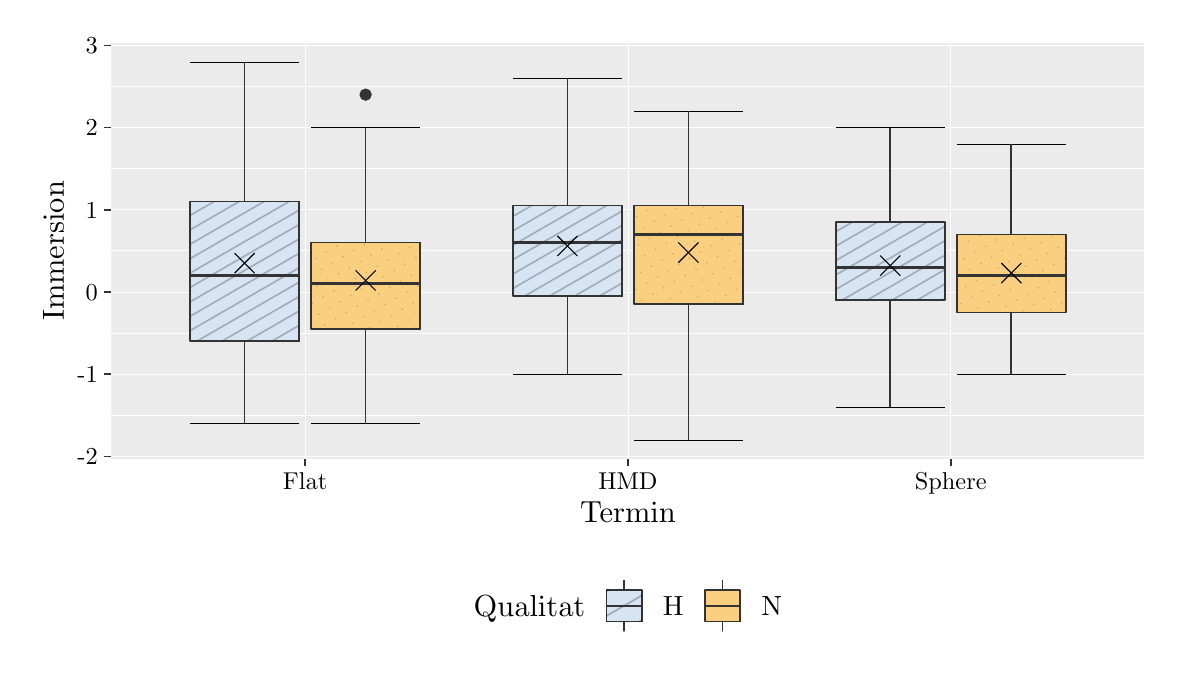
\begin{tikzpicture}[x=1pt,y=1pt]
\definecolor{fillColor}{RGB}{255,255,255}
\path[use as bounding box,fill=fillColor,fill opacity=0.00] (0,0) rectangle (409.05,231.26);
\begin{scope}
\path[clip] (  0.00,  0.00) rectangle (409.05,231.26);
\definecolor{drawColor}{RGB}{255,255,255}
\definecolor{fillColor}{RGB}{255,255,255}

\path[draw=drawColor,line width= 0.6pt,line join=round,line cap=round,fill=fillColor] (  0.00, -0.00) rectangle (409.05,231.26);
\end{scope}
\begin{scope}
\path[clip] ( 30.25, 75.45) rectangle (403.55,225.76);
\definecolor{fillColor}{gray}{0.92}

\path[fill=fillColor] ( 30.25, 75.45) rectangle (403.55,225.76);
\definecolor{drawColor}{RGB}{255,255,255}

\path[draw=drawColor,line width= 0.3pt,line join=round] ( 30.25, 91.19) --
	(403.55, 91.19);

\path[draw=drawColor,line width= 0.3pt,line join=round] ( 30.25,120.90) --
	(403.55,120.90);

\path[draw=drawColor,line width= 0.3pt,line join=round] ( 30.25,150.61) --
	(403.55,150.61);

\path[draw=drawColor,line width= 0.3pt,line join=round] ( 30.25,180.31) --
	(403.55,180.31);

\path[draw=drawColor,line width= 0.3pt,line join=round] ( 30.25,210.02) --
	(403.55,210.02);

\path[draw=drawColor,line width= 0.3pt,line join=round] ( 30.25, 76.34) --
	(403.55, 76.34);

\path[draw=drawColor,line width= 0.3pt,line join=round] ( 30.25,106.05) --
	(403.55,106.05);

\path[draw=drawColor,line width= 0.3pt,line join=round] ( 30.25,135.75) --
	(403.55,135.75);

\path[draw=drawColor,line width= 0.3pt,line join=round] ( 30.25,165.46) --
	(403.55,165.46);

\path[draw=drawColor,line width= 0.3pt,line join=round] ( 30.25,195.17) --
	(403.55,195.17);

\path[draw=drawColor,line width= 0.3pt,line join=round] ( 30.25,224.87) --
	(403.55,224.87);

\path[draw=drawColor,line width= 0.3pt,line join=round] (100.24, 75.45) --
	(100.24,225.76);

\path[draw=drawColor,line width= 0.3pt,line join=round] (216.90, 75.45) --
	(216.90,225.76);

\path[draw=drawColor,line width= 0.3pt,line join=round] (333.55, 75.45) --
	(333.55,225.76);
\definecolor{drawColor}{RGB}{0,0,0}

\path[draw=drawColor,line width= 0.2pt,line join=round] ( 58.68,218.93) --
	( 98.05,218.93);

\path[draw=drawColor,line width= 0.2pt,line join=round] ( 78.37,218.93) --
	( 78.37, 88.22);

\path[draw=drawColor,line width= 0.2pt,line join=round] ( 58.68, 88.22) --
	( 98.05, 88.22);

\path[draw=drawColor,line width= 0.2pt,line join=round] (102.43,195.17) --
	(141.80,195.17);

\path[draw=drawColor,line width= 0.2pt,line join=round] (122.11,195.17) --
	(122.11, 88.22);

\path[draw=drawColor,line width= 0.2pt,line join=round] (102.43, 88.22) --
	(141.80, 88.22);

\path[draw=drawColor,line width= 0.2pt,line join=round] (175.34,212.99) --
	(214.71,212.99);

\path[draw=drawColor,line width= 0.2pt,line join=round] (195.02,212.99) --
	(195.02,106.05);

\path[draw=drawColor,line width= 0.2pt,line join=round] (175.34,106.05) --
	(214.71,106.05);

\path[draw=drawColor,line width= 0.2pt,line join=round] (219.08,201.11) --
	(258.46,201.11);

\path[draw=drawColor,line width= 0.2pt,line join=round] (238.77,201.11) --
	(238.77, 82.28);

\path[draw=drawColor,line width= 0.2pt,line join=round] (219.08, 82.28) --
	(258.46, 82.28);

\path[draw=drawColor,line width= 0.2pt,line join=round] (291.99,195.17) --
	(331.37,195.17);

\path[draw=drawColor,line width= 0.2pt,line join=round] (311.68,195.17) --
	(311.68, 94.16);

\path[draw=drawColor,line width= 0.2pt,line join=round] (291.99, 94.16) --
	(331.37, 94.16);

\path[draw=drawColor,line width= 0.2pt,line join=round] (335.74,189.22) --
	(375.11,189.22);

\path[draw=drawColor,line width= 0.2pt,line join=round] (355.43,189.22) --
	(355.43,106.05);

\path[draw=drawColor,line width= 0.2pt,line join=round] (335.74,106.05) --
	(375.11,106.05);
\definecolor{drawColor}{gray}{0.20}

\path[draw=drawColor,line width= 0.2pt,line join=round] ( 78.37,168.43) -- ( 78.37,218.93);

\path[draw=drawColor,line width= 0.2pt,line join=round] ( 78.37,117.93) -- ( 78.37, 88.22);
\definecolor{fillColor}{RGB}{215,228,244}

\path[draw=drawColor,line width= 0.2pt,fill=fillColor] ( 58.68,168.43) --
	( 58.68,117.93) --
	( 98.05,117.93) --
	( 98.05,168.43) --
	( 58.68,168.43) --
	cycle;

\path[draw=drawColor,line width= 0.5pt] ( 58.68,141.69) -- ( 98.05,141.69);
\definecolor{fillColor}{gray}{0.20}

\path[draw=drawColor,line width= 0.4pt,line join=round,line cap=round,fill=fillColor] (122.11,207.05) circle (  1.96);

\path[draw=drawColor,line width= 0.2pt,line join=round] (122.11,153.58) -- (122.11,195.17);

\path[draw=drawColor,line width= 0.2pt,line join=round] (122.11,122.38) -- (122.11, 88.22);
\definecolor{fillColor}{RGB}{250,208,128}

\path[draw=drawColor,line width= 0.2pt,fill=fillColor] (102.43,153.58) --
	(102.43,122.38) --
	(141.80,122.38) --
	(141.80,153.58) --
	(102.43,153.58) --
	cycle;

\path[draw=drawColor,line width= 0.5pt] (102.43,138.72) -- (141.80,138.72);

\path[draw=drawColor,line width= 0.2pt,line join=round] (195.02,166.94) -- (195.02,212.99);

\path[draw=drawColor,line width= 0.2pt,line join=round] (195.02,134.27) -- (195.02,106.05);
\definecolor{fillColor}{RGB}{215,228,244}

\path[draw=drawColor,line width= 0.2pt,fill=fillColor] (175.34,166.94) --
	(175.34,134.27) --
	(214.71,134.27) --
	(214.71,166.94) --
	(175.34,166.94) --
	cycle;

\path[draw=drawColor,line width= 0.5pt] (175.34,153.58) -- (214.71,153.58);

\path[draw=drawColor,line width= 0.2pt,line join=round] (238.77,166.94) -- (238.77,201.11);

\path[draw=drawColor,line width= 0.2pt,line join=round] (238.77,131.30) -- (238.77, 82.28);
\definecolor{fillColor}{RGB}{250,208,128}

\path[draw=drawColor,line width= 0.2pt,fill=fillColor] (219.08,166.94) --
	(219.08,131.30) --
	(258.46,131.30) --
	(258.46,166.94) --
	(219.08,166.94) --
	cycle;

\path[draw=drawColor,line width= 0.5pt] (219.08,156.55) -- (258.46,156.55);

\path[draw=drawColor,line width= 0.2pt,line join=round] (311.68,161.00) -- (311.68,195.17);

\path[draw=drawColor,line width= 0.2pt,line join=round] (311.68,132.78) -- (311.68, 94.16);
\definecolor{fillColor}{RGB}{215,228,244}

\path[draw=drawColor,line width= 0.2pt,fill=fillColor] (291.99,161.00) --
	(291.99,132.78) --
	(331.37,132.78) --
	(331.37,161.00) --
	(291.99,161.00) --
	cycle;

\path[draw=drawColor,line width= 0.5pt] (291.99,144.66) -- (331.37,144.66);

\path[draw=drawColor,line width= 0.2pt,line join=round] (355.43,156.55) -- (355.43,189.22);

\path[draw=drawColor,line width= 0.2pt,line join=round] (355.43,128.33) -- (355.43,106.05);
\definecolor{fillColor}{RGB}{250,208,128}

\path[draw=drawColor,line width= 0.2pt,fill=fillColor] (335.74,156.55) --
	(335.74,128.33) --
	(375.11,128.33) --
	(375.11,156.55) --
	(335.74,156.55) --
	cycle;

\path[draw=drawColor,line width= 0.5pt] (335.74,141.69) -- (375.11,141.69);

\path[draw=drawColor,line width= 0.6pt,line join=round] ( 78.37,168.43) -- ( 78.37,218.93);

\path[draw=drawColor,line width= 0.6pt,line join=round] ( 78.37,117.93) -- ( 78.37, 88.22);
\definecolor{fillColor}{RGB}{215,228,244}

\path[fill=fillColor] ( 58.68,168.43) --
	( 58.68,117.93) --
	( 98.05,117.93) --
	( 98.05,168.43) --
	( 58.68,168.43) --
	cycle;
\definecolor{drawColor}{RGB}{0,0,0}
\definecolor{fillColor}{RGB}{0,0,0}

\path[draw=drawColor,draw opacity=0.20,line width= 0.6pt,line join=round,line cap=rect,fill=fillColor,fill opacity=0.20] ( 98.05,118.47) --
	( 98.05,118.41) --
	( 97.21,117.93) --
	( 97.12,117.93) --
	( 98.05,118.47) --
	cycle;

\path[draw=drawColor,draw opacity=0.20,line width= 0.6pt,line join=round,line cap=rect,fill=fillColor,fill opacity=0.20] ( 98.05,123.67) --
	( 98.05,123.62) --
	( 88.19,117.93) --
	( 88.10,117.93) --
	( 98.05,123.67) --
	cycle;

\path[draw=drawColor,draw opacity=0.20,line width= 0.6pt,line join=round,line cap=rect,fill=fillColor,fill opacity=0.20] ( 98.05,128.88) --
	( 98.05,128.83) --
	( 79.17,117.93) --
	( 79.08,117.93) --
	( 98.05,128.88) --
	cycle;

\path[draw=drawColor,draw opacity=0.20,line width= 0.6pt,line join=round,line cap=rect,fill=fillColor,fill opacity=0.20] ( 98.05,134.09) --
	( 98.05,134.04) --
	( 70.15,117.93) --
	( 70.06,117.93) --
	( 98.05,134.09) --
	cycle;

\path[draw=drawColor,draw opacity=0.20,line width= 0.6pt,line join=round,line cap=rect,fill=fillColor,fill opacity=0.20] ( 98.05,139.30) --
	( 98.05,139.24) --
	( 61.13,117.93) --
	( 61.04,117.93) --
	( 98.05,139.30) --
	cycle;

\path[draw=drawColor,draw opacity=0.20,line width= 0.6pt,line join=round,line cap=rect,fill=fillColor,fill opacity=0.20] ( 98.05,144.50) --
	( 98.05,144.45) --
	( 58.68,121.72) --
	( 58.68,121.77) --
	( 98.05,144.50) --
	cycle;

\path[draw=drawColor,draw opacity=0.20,line width= 0.6pt,line join=round,line cap=rect,fill=fillColor,fill opacity=0.20] ( 98.05,149.71) --
	( 98.05,149.66) --
	( 58.68,126.93) --
	( 58.68,126.98) --
	( 98.05,149.71) --
	cycle;

\path[draw=drawColor,draw opacity=0.20,line width= 0.6pt,line join=round,line cap=rect,fill=fillColor,fill opacity=0.20] ( 98.05,154.92) --
	( 98.05,154.86) --
	( 58.68,132.13) --
	( 58.68,132.19) --
	( 98.05,154.92) --
	cycle;

\path[draw=drawColor,draw opacity=0.20,line width= 0.6pt,line join=round,line cap=rect,fill=fillColor,fill opacity=0.20] ( 98.05,160.12) --
	( 98.05,160.07) --
	( 58.68,137.34) --
	( 58.68,137.39) --
	( 98.05,160.12) --
	cycle;

\path[draw=drawColor,draw opacity=0.20,line width= 0.6pt,line join=round,line cap=rect,fill=fillColor,fill opacity=0.20] ( 98.05,165.33) --
	( 98.05,165.28) --
	( 58.68,142.55) --
	( 58.68,142.60) --
	( 98.05,165.33) --
	cycle;

\path[draw=drawColor,draw opacity=0.20,line width= 0.6pt,line join=round,line cap=rect,fill=fillColor,fill opacity=0.20] ( 94.40,168.43) --
	( 94.49,168.43) --
	( 58.68,147.75) --
	( 58.68,147.81) --
	( 94.40,168.43) --
	cycle;

\path[draw=drawColor,draw opacity=0.20,line width= 0.6pt,line join=round,line cap=rect,fill=fillColor,fill opacity=0.20] ( 85.38,168.43) --
	( 85.47,168.43) --
	( 58.68,152.96) --
	( 58.68,153.01) --
	( 85.38,168.43) --
	cycle;

\path[draw=drawColor,draw opacity=0.20,line width= 0.6pt,line join=round,line cap=rect,fill=fillColor,fill opacity=0.20] ( 76.36,168.43) --
	( 76.45,168.43) --
	( 58.68,158.17) --
	( 58.68,158.22) --
	( 76.36,168.43) --
	cycle;

\path[draw=drawColor,draw opacity=0.20,line width= 0.6pt,line join=round,line cap=rect,fill=fillColor,fill opacity=0.20] ( 67.34,168.43) --
	( 67.44,168.43) --
	( 58.68,163.38) --
	( 58.68,163.43) --
	( 67.34,168.43) --
	cycle;
\definecolor{drawColor}{gray}{0.20}

\path[draw=drawColor,line width= 0.6pt,line join=round,line cap=round] ( 58.68,168.43) --
	( 58.68,117.93) --
	( 98.05,117.93) --
	( 98.05,168.43) --
	( 58.68,168.43) --
	cycle;

\path[draw=drawColor,line width= 1.1pt,line join=round] ( 58.68,141.69) -- ( 98.05,141.69);

\path[draw=drawColor,line width= 0.6pt,line join=round] (195.02,166.94) -- (195.02,212.99);

\path[draw=drawColor,line width= 0.6pt,line join=round] (195.02,134.27) -- (195.02,106.05);
\definecolor{fillColor}{RGB}{215,228,244}

\path[fill=fillColor] (175.34,166.94) --
	(175.34,134.27) --
	(214.71,134.27) --
	(214.71,166.94) --
	(175.34,166.94) --
	cycle;
\definecolor{drawColor}{RGB}{0,0,0}
\definecolor{fillColor}{RGB}{0,0,0}

\path[draw=drawColor,draw opacity=0.20,line width= 0.6pt,line join=round,line cap=rect,fill=fillColor,fill opacity=0.20] (214.71,138.95) --
	(214.71,138.90) --
	(206.68,134.27) --
	(206.59,134.27) --
	(214.71,138.95) --
	cycle;

\path[draw=drawColor,draw opacity=0.20,line width= 0.6pt,line join=round,line cap=rect,fill=fillColor,fill opacity=0.20] (214.71,144.16) --
	(214.71,144.11) --
	(197.66,134.27) --
	(197.57,134.27) --
	(214.71,144.16) --
	cycle;

\path[draw=drawColor,draw opacity=0.20,line width= 0.6pt,line join=round,line cap=rect,fill=fillColor,fill opacity=0.20] (214.71,149.37) --
	(214.71,149.32) --
	(188.64,134.27) --
	(188.55,134.27) --
	(214.71,149.37) --
	cycle;

\path[draw=drawColor,draw opacity=0.20,line width= 0.6pt,line join=round,line cap=rect,fill=fillColor,fill opacity=0.20] (214.71,154.58) --
	(214.71,154.52) --
	(179.62,134.27) --
	(179.53,134.27) --
	(214.71,154.58) --
	cycle;

\path[draw=drawColor,draw opacity=0.20,line width= 0.6pt,line join=round,line cap=rect,fill=fillColor,fill opacity=0.20] (214.71,159.78) --
	(214.71,159.73) --
	(175.34,137.00) --
	(175.34,137.05) --
	(214.71,159.78) --
	cycle;

\path[draw=drawColor,draw opacity=0.20,line width= 0.6pt,line join=round,line cap=rect,fill=fillColor,fill opacity=0.20] (214.71,164.99) --
	(214.71,164.94) --
	(175.34,142.21) --
	(175.34,142.26) --
	(214.71,164.99) --
	cycle;

\path[draw=drawColor,draw opacity=0.20,line width= 0.6pt,line join=round,line cap=rect,fill=fillColor,fill opacity=0.20] (209.08,166.94) --
	(209.17,166.94) --
	(175.34,147.41) --
	(175.34,147.47) --
	(209.08,166.94) --
	cycle;

\path[draw=drawColor,draw opacity=0.20,line width= 0.6pt,line join=round,line cap=rect,fill=fillColor,fill opacity=0.20] (200.06,166.94) --
	(200.15,166.94) --
	(175.34,152.62) --
	(175.34,152.67) --
	(200.06,166.94) --
	cycle;

\path[draw=drawColor,draw opacity=0.20,line width= 0.6pt,line join=round,line cap=rect,fill=fillColor,fill opacity=0.20] (191.04,166.94) --
	(191.13,166.94) --
	(175.34,157.83) --
	(175.34,157.88) --
	(191.04,166.94) --
	cycle;

\path[draw=drawColor,draw opacity=0.20,line width= 0.6pt,line join=round,line cap=rect,fill=fillColor,fill opacity=0.20] (182.02,166.94) --
	(182.11,166.94) --
	(175.34,163.04) --
	(175.34,163.09) --
	(182.02,166.94) --
	cycle;
\definecolor{drawColor}{gray}{0.20}

\path[draw=drawColor,line width= 0.6pt,line join=round,line cap=round] (175.34,166.94) --
	(175.34,134.27) --
	(214.71,134.27) --
	(214.71,166.94) --
	(175.34,166.94) --
	cycle;

\path[draw=drawColor,line width= 1.1pt,line join=round] (175.34,153.58) -- (214.71,153.58);

\path[draw=drawColor,line width= 0.6pt,line join=round] (311.68,161.00) -- (311.68,195.17);

\path[draw=drawColor,line width= 0.6pt,line join=round] (311.68,132.78) -- (311.68, 94.16);
\definecolor{fillColor}{RGB}{215,228,244}

\path[fill=fillColor] (291.99,161.00) --
	(291.99,132.78) --
	(331.37,132.78) --
	(331.37,161.00) --
	(291.99,161.00) --
	cycle;
\definecolor{drawColor}{RGB}{0,0,0}
\definecolor{fillColor}{RGB}{0,0,0}

\path[draw=drawColor,draw opacity=0.20,line width= 0.6pt,line join=round,line cap=rect,fill=fillColor,fill opacity=0.20] (331.37,133.41) --
	(331.37,133.36) --
	(330.37,132.78) --
	(330.28,132.78) --
	(331.37,133.41) --
	cycle;

\path[draw=drawColor,draw opacity=0.20,line width= 0.6pt,line join=round,line cap=rect,fill=fillColor,fill opacity=0.20] (331.37,138.61) --
	(331.37,138.56) --
	(321.35,132.78) --
	(321.26,132.78) --
	(331.37,138.61) --
	cycle;

\path[draw=drawColor,draw opacity=0.20,line width= 0.6pt,line join=round,line cap=rect,fill=fillColor,fill opacity=0.20] (331.37,143.82) --
	(331.37,143.77) --
	(312.34,132.78) --
	(312.25,132.78) --
	(331.37,143.82) --
	cycle;

\path[draw=drawColor,draw opacity=0.20,line width= 0.6pt,line join=round,line cap=rect,fill=fillColor,fill opacity=0.20] (331.37,149.03) --
	(331.37,148.98) --
	(303.32,132.78) --
	(303.23,132.78) --
	(331.37,149.03) --
	cycle;

\path[draw=drawColor,draw opacity=0.20,line width= 0.6pt,line join=round,line cap=rect,fill=fillColor,fill opacity=0.20] (331.37,154.24) --
	(331.37,154.18) --
	(294.30,132.78) --
	(294.21,132.78) --
	(331.37,154.24) --
	cycle;

\path[draw=drawColor,draw opacity=0.20,line width= 0.6pt,line join=round,line cap=rect,fill=fillColor,fill opacity=0.20] (331.37,159.44) --
	(331.37,159.39) --
	(291.99,136.66) --
	(291.99,136.71) --
	(331.37,159.44) --
	cycle;

\path[draw=drawColor,draw opacity=0.20,line width= 0.6pt,line join=round,line cap=rect,fill=fillColor,fill opacity=0.20] (325.05,161.00) --
	(325.14,161.00) --
	(291.99,141.87) --
	(291.99,141.92) --
	(325.05,161.00) --
	cycle;

\path[draw=drawColor,draw opacity=0.20,line width= 0.6pt,line join=round,line cap=rect,fill=fillColor,fill opacity=0.20] (316.03,161.00) --
	(316.12,161.00) --
	(291.99,147.07) --
	(291.99,147.13) --
	(316.03,161.00) --
	cycle;

\path[draw=drawColor,draw opacity=0.20,line width= 0.6pt,line join=round,line cap=rect,fill=fillColor,fill opacity=0.20] (307.01,161.00) --
	(307.10,161.00) --
	(291.99,152.28) --
	(291.99,152.33) --
	(307.01,161.00) --
	cycle;

\path[draw=drawColor,draw opacity=0.20,line width= 0.6pt,line join=round,line cap=rect,fill=fillColor,fill opacity=0.20] (297.99,161.00) --
	(298.08,161.00) --
	(291.99,157.49) --
	(291.99,157.54) --
	(297.99,161.00) --
	cycle;
\definecolor{drawColor}{gray}{0.20}

\path[draw=drawColor,line width= 0.6pt,line join=round,line cap=round] (291.99,161.00) --
	(291.99,132.78) --
	(331.37,132.78) --
	(331.37,161.00) --
	(291.99,161.00) --
	cycle;

\path[draw=drawColor,line width= 1.1pt,line join=round] (291.99,144.66) -- (331.37,144.66);
\definecolor{fillColor}{gray}{0.20}

\path[draw=drawColor,line width= 0.4pt,line join=round,line cap=round,fill=fillColor] (122.11,207.05) circle (  1.96);

\path[draw=drawColor,line width= 0.6pt,line join=round] (122.11,153.58) -- (122.11,195.17);

\path[draw=drawColor,line width= 0.6pt,line join=round] (122.11,122.38) -- (122.11, 88.22);
\definecolor{fillColor}{RGB}{250,208,128}

\path[fill=fillColor] (102.43,153.58) --
	(102.43,122.38) --
	(141.80,122.38) --
	(141.80,153.58) --
	(102.43,153.58) --
	cycle;
\definecolor{drawColor}{RGB}{0,0,0}
\definecolor{fillColor}{RGB}{0,0,0}

\path[draw=drawColor,draw opacity=0.20,line width= 0.6pt,line join=round,line cap=round,fill=fillColor,fill opacity=0.20] (102.88,131.64) circle (  0.02);

\path[draw=drawColor,draw opacity=0.20,line width= 0.6pt,line join=round,line cap=round,fill=fillColor,fill opacity=0.20] (103.92,147.87) circle (  0.02);

\path[draw=drawColor,draw opacity=0.20,line width= 0.6pt,line join=round,line cap=round,fill=fillColor,fill opacity=0.20] (104.53,137.80) circle (  0.02);

\path[draw=drawColor,draw opacity=0.20,line width= 0.6pt,line join=round,line cap=round,fill=fillColor,fill opacity=0.20] (105.13,127.73) circle (  0.02);

\path[draw=drawColor,draw opacity=0.20,line width= 0.6pt,line join=round,line cap=round,fill=fillColor,fill opacity=0.20] (106.18,143.96) circle (  0.02);

\path[draw=drawColor,draw opacity=0.20,line width= 0.6pt,line join=round,line cap=round,fill=fillColor,fill opacity=0.20] (106.78,133.89) circle (  0.02);

\path[draw=drawColor,draw opacity=0.20,line width= 0.6pt,line join=round,line cap=round,fill=fillColor,fill opacity=0.20] (107.39,123.83) circle (  0.02);

\path[draw=drawColor,draw opacity=0.20,line width= 0.6pt,line join=round,line cap=round,fill=fillColor,fill opacity=0.20] (107.83,150.12) circle (  0.02);

\path[draw=drawColor,draw opacity=0.20,line width= 0.6pt,line join=round,line cap=round,fill=fillColor,fill opacity=0.20] (108.43,140.05) circle (  0.02);

\path[draw=drawColor,draw opacity=0.20,line width= 0.6pt,line join=round,line cap=round,fill=fillColor,fill opacity=0.20] (109.04,129.99) circle (  0.02);

\path[draw=drawColor,draw opacity=0.20,line width= 0.6pt,line join=round,line cap=round,fill=fillColor,fill opacity=0.20] (110.08,146.22) circle (  0.02);

\path[draw=drawColor,draw opacity=0.20,line width= 0.6pt,line join=round,line cap=round,fill=fillColor,fill opacity=0.20] (110.69,136.15) circle (  0.02);

\path[draw=drawColor,draw opacity=0.20,line width= 0.6pt,line join=round,line cap=round,fill=fillColor,fill opacity=0.20] (111.29,126.08) circle (  0.02);

\path[draw=drawColor,draw opacity=0.20,line width= 0.6pt,line join=round,line cap=round,fill=fillColor,fill opacity=0.20] (111.73,152.38) circle (  0.02);

\path[draw=drawColor,draw opacity=0.20,line width= 0.6pt,line join=round,line cap=round,fill=fillColor,fill opacity=0.20] (112.34,142.31) circle (  0.02);

\path[draw=drawColor,draw opacity=0.20,line width= 0.6pt,line join=round,line cap=round,fill=fillColor,fill opacity=0.20] (112.94,132.24) circle (  0.02);

\path[draw=drawColor,draw opacity=0.20,line width= 0.6pt,line join=round,line cap=round,fill=fillColor,fill opacity=0.20] (113.99,148.47) circle (  0.02);

\path[draw=drawColor,draw opacity=0.20,line width= 0.6pt,line join=round,line cap=round,fill=fillColor,fill opacity=0.20] (114.59,138.40) circle (  0.02);

\path[draw=drawColor,draw opacity=0.20,line width= 0.6pt,line join=round,line cap=round,fill=fillColor,fill opacity=0.20] (115.20,128.34) circle (  0.02);

\path[draw=drawColor,draw opacity=0.20,line width= 0.6pt,line join=round,line cap=round,fill=fillColor,fill opacity=0.20] (116.24,144.56) circle (  0.02);

\path[draw=drawColor,draw opacity=0.20,line width= 0.6pt,line join=round,line cap=round,fill=fillColor,fill opacity=0.20] (116.85,134.50) circle (  0.02);

\path[draw=drawColor,draw opacity=0.20,line width= 0.6pt,line join=round,line cap=round,fill=fillColor,fill opacity=0.20] (117.45,124.43) circle (  0.02);

\path[draw=drawColor,draw opacity=0.20,line width= 0.6pt,line join=round,line cap=round,fill=fillColor,fill opacity=0.20] (117.89,150.72) circle (  0.02);

\path[draw=drawColor,draw opacity=0.20,line width= 0.6pt,line join=round,line cap=round,fill=fillColor,fill opacity=0.20] (118.50,140.66) circle (  0.02);

\path[draw=drawColor,draw opacity=0.20,line width= 0.6pt,line join=round,line cap=round,fill=fillColor,fill opacity=0.20] (119.10,130.59) circle (  0.02);

\path[draw=drawColor,draw opacity=0.20,line width= 0.6pt,line join=round,line cap=round,fill=fillColor,fill opacity=0.20] (120.15,146.82) circle (  0.02);

\path[draw=drawColor,draw opacity=0.20,line width= 0.6pt,line join=round,line cap=round,fill=fillColor,fill opacity=0.20] (120.75,136.75) circle (  0.02);

\path[draw=drawColor,draw opacity=0.20,line width= 0.6pt,line join=round,line cap=round,fill=fillColor,fill opacity=0.20] (121.36,126.69) circle (  0.02);

\path[draw=drawColor,draw opacity=0.20,line width= 0.6pt,line join=round,line cap=round,fill=fillColor,fill opacity=0.20] (121.80,152.98) circle (  0.02);

\path[draw=drawColor,draw opacity=0.20,line width= 0.6pt,line join=round,line cap=round,fill=fillColor,fill opacity=0.20] (122.40,142.91) circle (  0.02);

\path[draw=drawColor,draw opacity=0.20,line width= 0.6pt,line join=round,line cap=round,fill=fillColor,fill opacity=0.20] (123.01,132.85) circle (  0.02);

\path[draw=drawColor,draw opacity=0.20,line width= 0.6pt,line join=round,line cap=round,fill=fillColor,fill opacity=0.20] (123.61,122.78) circle (  0.02);

\path[draw=drawColor,draw opacity=0.20,line width= 0.6pt,line join=round,line cap=round,fill=fillColor,fill opacity=0.20] (124.05,149.07) circle (  0.02);

\path[draw=drawColor,draw opacity=0.20,line width= 0.6pt,line join=round,line cap=round,fill=fillColor,fill opacity=0.20] (124.66,139.01) circle (  0.02);

\path[draw=drawColor,draw opacity=0.20,line width= 0.6pt,line join=round,line cap=round,fill=fillColor,fill opacity=0.20] (125.26,128.94) circle (  0.02);

\path[draw=drawColor,draw opacity=0.20,line width= 0.6pt,line join=round,line cap=round,fill=fillColor,fill opacity=0.20] (126.31,145.17) circle (  0.02);

\path[draw=drawColor,draw opacity=0.20,line width= 0.6pt,line join=round,line cap=round,fill=fillColor,fill opacity=0.20] (126.91,135.10) circle (  0.02);

\path[draw=drawColor,draw opacity=0.20,line width= 0.6pt,line join=round,line cap=round,fill=fillColor,fill opacity=0.20] (127.52,125.04) circle (  0.02);

\path[draw=drawColor,draw opacity=0.20,line width= 0.6pt,line join=round,line cap=round,fill=fillColor,fill opacity=0.20] (127.96,151.33) circle (  0.02);

\path[draw=drawColor,draw opacity=0.20,line width= 0.6pt,line join=round,line cap=round,fill=fillColor,fill opacity=0.20] (128.56,141.26) circle (  0.02);

\path[draw=drawColor,draw opacity=0.20,line width= 0.6pt,line join=round,line cap=round,fill=fillColor,fill opacity=0.20] (129.17,131.20) circle (  0.02);

\path[draw=drawColor,draw opacity=0.20,line width= 0.6pt,line join=round,line cap=round,fill=fillColor,fill opacity=0.20] (130.21,147.42) circle (  0.02);

\path[draw=drawColor,draw opacity=0.20,line width= 0.6pt,line join=round,line cap=round,fill=fillColor,fill opacity=0.20] (130.82,137.36) circle (  0.02);

\path[draw=drawColor,draw opacity=0.20,line width= 0.6pt,line join=round,line cap=round,fill=fillColor,fill opacity=0.20] (131.42,127.29) circle (  0.02);

\path[draw=drawColor,draw opacity=0.20,line width= 0.6pt,line join=round,line cap=round,fill=fillColor,fill opacity=0.20] (132.47,143.52) circle (  0.02);

\path[draw=drawColor,draw opacity=0.20,line width= 0.6pt,line join=round,line cap=round,fill=fillColor,fill opacity=0.20] (133.07,133.45) circle (  0.02);

\path[draw=drawColor,draw opacity=0.20,line width= 0.6pt,line join=round,line cap=round,fill=fillColor,fill opacity=0.20] (133.68,123.39) circle (  0.02);

\path[draw=drawColor,draw opacity=0.20,line width= 0.6pt,line join=round,line cap=round,fill=fillColor,fill opacity=0.20] (134.12,149.68) circle (  0.02);

\path[draw=drawColor,draw opacity=0.20,line width= 0.6pt,line join=round,line cap=round,fill=fillColor,fill opacity=0.20] (134.72,139.61) circle (  0.02);

\path[draw=drawColor,draw opacity=0.20,line width= 0.6pt,line join=round,line cap=round,fill=fillColor,fill opacity=0.20] (135.33,129.55) circle (  0.02);

\path[draw=drawColor,draw opacity=0.20,line width= 0.6pt,line join=round,line cap=round,fill=fillColor,fill opacity=0.20] (136.37,145.77) circle (  0.02);

\path[draw=drawColor,draw opacity=0.20,line width= 0.6pt,line join=round,line cap=round,fill=fillColor,fill opacity=0.20] (136.98,135.71) circle (  0.02);

\path[draw=drawColor,draw opacity=0.20,line width= 0.6pt,line join=round,line cap=round,fill=fillColor,fill opacity=0.20] (137.58,125.64) circle (  0.02);

\path[draw=drawColor,draw opacity=0.20,line width= 0.6pt,line join=round,line cap=round,fill=fillColor,fill opacity=0.20] (138.02,151.93) circle (  0.02);

\path[draw=drawColor,draw opacity=0.20,line width= 0.6pt,line join=round,line cap=round,fill=fillColor,fill opacity=0.20] (138.63,141.87) circle (  0.02);

\path[draw=drawColor,draw opacity=0.20,line width= 0.6pt,line join=round,line cap=round,fill=fillColor,fill opacity=0.20] (139.23,131.80) circle (  0.02);

\path[draw=drawColor,draw opacity=0.20,line width= 0.6pt,line join=round,line cap=round,fill=fillColor,fill opacity=0.20] (140.28,148.03) circle (  0.02);

\path[draw=drawColor,draw opacity=0.20,line width= 0.6pt,line join=round,line cap=round,fill=fillColor,fill opacity=0.20] (140.88,137.96) circle (  0.02);

\path[draw=drawColor,draw opacity=0.20,line width= 0.6pt,line join=round,line cap=round,fill=fillColor,fill opacity=0.20] (141.49,127.90) circle (  0.02);

\path[draw=drawColor,draw opacity=0.20,line width= 0.6pt,line join=round,line cap=round,fill=fillColor,fill opacity=0.20] (131.89,153.58) --
	(131.89,153.57) --
	(131.88,153.57) --
	(131.88,153.57) --
	(131.88,153.57) --
	(131.88,153.57) --
	(131.88,153.57) --
	(131.88,153.57) --
	(131.88,153.57) --
	(131.88,153.57) --
	(131.88,153.56) --
	(131.88,153.56) --
	(131.87,153.56) --
	(131.87,153.56) --
	(131.87,153.56) --
	(131.87,153.56) --
	(131.87,153.56) --
	(131.87,153.56) --
	(131.87,153.56) --
	(131.86,153.56) --
	(131.86,153.56) --
	(131.86,153.56) --
	(131.86,153.56) --
	(131.86,153.56) --
	(131.86,153.56) --
	(131.86,153.56) --
	(131.86,153.56) --
	(131.85,153.56) --
	(131.85,153.56) --
	(131.85,153.56) --
	(131.85,153.57) --
	(131.85,153.57) --
	(131.85,153.57) --
	(131.85,153.57) --
	(131.85,153.57) --
	(131.85,153.57) --
	(131.84,153.57) --
	(131.84,153.57) --
	(131.84,153.57) --
	(131.84,153.58) --
	(131.84,153.58) --
	(131.89,153.58) --
	(131.89,153.58) --
	cycle;
\definecolor{drawColor}{gray}{0.20}

\path[draw=drawColor,line width= 0.6pt,line join=round,line cap=round] (102.43,153.58) --
	(102.43,122.38) --
	(141.80,122.38) --
	(141.80,153.58) --
	(102.43,153.58) --
	cycle;

\path[draw=drawColor,line width= 1.1pt,line join=round] (102.43,138.72) -- (141.80,138.72);

\path[draw=drawColor,line width= 0.6pt,line join=round] (238.77,166.94) -- (238.77,201.11);

\path[draw=drawColor,line width= 0.6pt,line join=round] (238.77,131.30) -- (238.77, 82.28);
\definecolor{fillColor}{RGB}{250,208,128}

\path[fill=fillColor] (219.08,166.94) --
	(219.08,131.30) --
	(258.46,131.30) --
	(258.46,166.94) --
	(219.08,166.94) --
	cycle;
\definecolor{drawColor}{RGB}{0,0,0}
\definecolor{fillColor}{RGB}{0,0,0}

\path[draw=drawColor,draw opacity=0.20,line width= 0.6pt,line join=round,line cap=round,fill=fillColor,fill opacity=0.20] (219.15,146.70) circle (  0.02);

\path[draw=drawColor,draw opacity=0.20,line width= 0.6pt,line join=round,line cap=round,fill=fillColor,fill opacity=0.20] (219.76,136.64) circle (  0.02);

\path[draw=drawColor,draw opacity=0.20,line width= 0.6pt,line join=round,line cap=round,fill=fillColor,fill opacity=0.20] (220.20,162.93) circle (  0.02);

\path[draw=drawColor,draw opacity=0.20,line width= 0.6pt,line join=round,line cap=round,fill=fillColor,fill opacity=0.20] (220.80,152.86) circle (  0.02);

\path[draw=drawColor,draw opacity=0.20,line width= 0.6pt,line join=round,line cap=round,fill=fillColor,fill opacity=0.20] (221.41,142.80) circle (  0.02);

\path[draw=drawColor,draw opacity=0.20,line width= 0.6pt,line join=round,line cap=round,fill=fillColor,fill opacity=0.20] (222.01,132.73) circle (  0.02);

\path[draw=drawColor,draw opacity=0.20,line width= 0.6pt,line join=round,line cap=round,fill=fillColor,fill opacity=0.20] (222.45,159.02) circle (  0.02);

\path[draw=drawColor,draw opacity=0.20,line width= 0.6pt,line join=round,line cap=round,fill=fillColor,fill opacity=0.20] (223.06,148.96) circle (  0.02);

\path[draw=drawColor,draw opacity=0.20,line width= 0.6pt,line join=round,line cap=round,fill=fillColor,fill opacity=0.20] (223.66,138.89) circle (  0.02);

\path[draw=drawColor,draw opacity=0.20,line width= 0.6pt,line join=round,line cap=round,fill=fillColor,fill opacity=0.20] (224.10,165.18) circle (  0.02);

\path[draw=drawColor,draw opacity=0.20,line width= 0.6pt,line join=round,line cap=round,fill=fillColor,fill opacity=0.20] (224.71,155.12) circle (  0.02);

\path[draw=drawColor,draw opacity=0.20,line width= 0.6pt,line join=round,line cap=round,fill=fillColor,fill opacity=0.20] (225.31,145.05) circle (  0.02);

\path[draw=drawColor,draw opacity=0.20,line width= 0.6pt,line join=round,line cap=round,fill=fillColor,fill opacity=0.20] (225.92,134.98) circle (  0.02);

\path[draw=drawColor,draw opacity=0.20,line width= 0.6pt,line join=round,line cap=round,fill=fillColor,fill opacity=0.20] (226.36,161.28) circle (  0.02);

\path[draw=drawColor,draw opacity=0.20,line width= 0.6pt,line join=round,line cap=round,fill=fillColor,fill opacity=0.20] (226.96,151.21) circle (  0.02);

\path[draw=drawColor,draw opacity=0.20,line width= 0.6pt,line join=round,line cap=round,fill=fillColor,fill opacity=0.20] (227.57,141.14) circle (  0.02);

\path[draw=drawColor,draw opacity=0.20,line width= 0.6pt,line join=round,line cap=round,fill=fillColor,fill opacity=0.20] (228.61,157.37) circle (  0.02);

\path[draw=drawColor,draw opacity=0.20,line width= 0.6pt,line join=round,line cap=round,fill=fillColor,fill opacity=0.20] (229.22,147.30) circle (  0.02);

\path[draw=drawColor,draw opacity=0.20,line width= 0.6pt,line join=round,line cap=round,fill=fillColor,fill opacity=0.20] (229.82,137.24) circle (  0.02);

\path[draw=drawColor,draw opacity=0.20,line width= 0.6pt,line join=round,line cap=round,fill=fillColor,fill opacity=0.20] (230.26,163.53) circle (  0.02);

\path[draw=drawColor,draw opacity=0.20,line width= 0.6pt,line join=round,line cap=round,fill=fillColor,fill opacity=0.20] (230.87,153.46) circle (  0.02);

\path[draw=drawColor,draw opacity=0.20,line width= 0.6pt,line join=round,line cap=round,fill=fillColor,fill opacity=0.20] (231.47,143.40) circle (  0.02);

\path[draw=drawColor,draw opacity=0.20,line width= 0.6pt,line join=round,line cap=round,fill=fillColor,fill opacity=0.20] (232.08,133.33) circle (  0.02);

\path[draw=drawColor,draw opacity=0.20,line width= 0.6pt,line join=round,line cap=round,fill=fillColor,fill opacity=0.20] (232.52,159.62) circle (  0.02);

\path[draw=drawColor,draw opacity=0.20,line width= 0.6pt,line join=round,line cap=round,fill=fillColor,fill opacity=0.20] (233.12,149.56) circle (  0.02);

\path[draw=drawColor,draw opacity=0.20,line width= 0.6pt,line join=round,line cap=round,fill=fillColor,fill opacity=0.20] (233.73,139.49) circle (  0.02);

\path[draw=drawColor,draw opacity=0.20,line width= 0.6pt,line join=round,line cap=round,fill=fillColor,fill opacity=0.20] (234.17,165.79) circle (  0.02);

\path[draw=drawColor,draw opacity=0.20,line width= 0.6pt,line join=round,line cap=round,fill=fillColor,fill opacity=0.20] (234.77,155.72) circle (  0.02);

\path[draw=drawColor,draw opacity=0.20,line width= 0.6pt,line join=round,line cap=round,fill=fillColor,fill opacity=0.20] (235.38,145.65) circle (  0.02);

\path[draw=drawColor,draw opacity=0.20,line width= 0.6pt,line join=round,line cap=round,fill=fillColor,fill opacity=0.20] (235.98,135.59) circle (  0.02);

\path[draw=drawColor,draw opacity=0.20,line width= 0.6pt,line join=round,line cap=round,fill=fillColor,fill opacity=0.20] (236.42,161.88) circle (  0.02);

\path[draw=drawColor,draw opacity=0.20,line width= 0.6pt,line join=round,line cap=round,fill=fillColor,fill opacity=0.20] (237.03,151.81) circle (  0.02);

\path[draw=drawColor,draw opacity=0.20,line width= 0.6pt,line join=round,line cap=round,fill=fillColor,fill opacity=0.20] (237.63,141.75) circle (  0.02);

\path[draw=drawColor,draw opacity=0.20,line width= 0.6pt,line join=round,line cap=round,fill=fillColor,fill opacity=0.20] (238.24,131.68) circle (  0.02);

\path[draw=drawColor,draw opacity=0.20,line width= 0.6pt,line join=round,line cap=round,fill=fillColor,fill opacity=0.20] (238.68,157.97) circle (  0.02);

\path[draw=drawColor,draw opacity=0.20,line width= 0.6pt,line join=round,line cap=round,fill=fillColor,fill opacity=0.20] (239.28,147.91) circle (  0.02);

\path[draw=drawColor,draw opacity=0.20,line width= 0.6pt,line join=round,line cap=round,fill=fillColor,fill opacity=0.20] (239.89,137.84) circle (  0.02);

\path[draw=drawColor,draw opacity=0.20,line width= 0.6pt,line join=round,line cap=round,fill=fillColor,fill opacity=0.20] (240.33,164.13) circle (  0.02);

\path[draw=drawColor,draw opacity=0.20,line width= 0.6pt,line join=round,line cap=round,fill=fillColor,fill opacity=0.20] (240.93,154.07) circle (  0.02);

\path[draw=drawColor,draw opacity=0.20,line width= 0.6pt,line join=round,line cap=round,fill=fillColor,fill opacity=0.20] (241.54,144.00) circle (  0.02);

\path[draw=drawColor,draw opacity=0.20,line width= 0.6pt,line join=round,line cap=round,fill=fillColor,fill opacity=0.20] (242.14,133.94) circle (  0.02);

\path[draw=drawColor,draw opacity=0.20,line width= 0.6pt,line join=round,line cap=round,fill=fillColor,fill opacity=0.20] (242.58,160.23) circle (  0.02);

\path[draw=drawColor,draw opacity=0.20,line width= 0.6pt,line join=round,line cap=round,fill=fillColor,fill opacity=0.20] (243.19,150.16) circle (  0.02);

\path[draw=drawColor,draw opacity=0.20,line width= 0.6pt,line join=round,line cap=round,fill=fillColor,fill opacity=0.20] (243.79,140.10) circle (  0.02);

\path[draw=drawColor,draw opacity=0.20,line width= 0.6pt,line join=round,line cap=round,fill=fillColor,fill opacity=0.20] (244.23,166.39) circle (  0.02);

\path[draw=drawColor,draw opacity=0.20,line width= 0.6pt,line join=round,line cap=round,fill=fillColor,fill opacity=0.20] (244.84,156.32) circle (  0.02);

\path[draw=drawColor,draw opacity=0.20,line width= 0.6pt,line join=round,line cap=round,fill=fillColor,fill opacity=0.20] (245.44,146.26) circle (  0.02);

\path[draw=drawColor,draw opacity=0.20,line width= 0.6pt,line join=round,line cap=round,fill=fillColor,fill opacity=0.20] (246.05,136.19) circle (  0.02);

\path[draw=drawColor,draw opacity=0.20,line width= 0.6pt,line join=round,line cap=round,fill=fillColor,fill opacity=0.20] (246.49,162.48) circle (  0.02);

\path[draw=drawColor,draw opacity=0.20,line width= 0.6pt,line join=round,line cap=round,fill=fillColor,fill opacity=0.20] (247.09,152.42) circle (  0.02);

\path[draw=drawColor,draw opacity=0.20,line width= 0.6pt,line join=round,line cap=round,fill=fillColor,fill opacity=0.20] (247.70,142.35) circle (  0.02);

\path[draw=drawColor,draw opacity=0.20,line width= 0.6pt,line join=round,line cap=round,fill=fillColor,fill opacity=0.20] (248.30,132.29) circle (  0.02);

\path[draw=drawColor,draw opacity=0.20,line width= 0.6pt,line join=round,line cap=round,fill=fillColor,fill opacity=0.20] (248.74,158.58) circle (  0.02);

\path[draw=drawColor,draw opacity=0.20,line width= 0.6pt,line join=round,line cap=round,fill=fillColor,fill opacity=0.20] (249.35,148.51) circle (  0.02);

\path[draw=drawColor,draw opacity=0.20,line width= 0.6pt,line join=round,line cap=round,fill=fillColor,fill opacity=0.20] (249.95,138.45) circle (  0.02);

\path[draw=drawColor,draw opacity=0.20,line width= 0.6pt,line join=round,line cap=round,fill=fillColor,fill opacity=0.20] (250.39,164.74) circle (  0.02);

\path[draw=drawColor,draw opacity=0.20,line width= 0.6pt,line join=round,line cap=round,fill=fillColor,fill opacity=0.20] (251.00,154.67) circle (  0.02);

\path[draw=drawColor,draw opacity=0.20,line width= 0.6pt,line join=round,line cap=round,fill=fillColor,fill opacity=0.20] (251.60,144.61) circle (  0.02);

\path[draw=drawColor,draw opacity=0.20,line width= 0.6pt,line join=round,line cap=round,fill=fillColor,fill opacity=0.20] (252.21,134.54) circle (  0.02);

\path[draw=drawColor,draw opacity=0.20,line width= 0.6pt,line join=round,line cap=round,fill=fillColor,fill opacity=0.20] (252.65,160.83) circle (  0.02);

\path[draw=drawColor,draw opacity=0.20,line width= 0.6pt,line join=round,line cap=round,fill=fillColor,fill opacity=0.20] (253.25,150.77) circle (  0.02);

\path[draw=drawColor,draw opacity=0.20,line width= 0.6pt,line join=round,line cap=round,fill=fillColor,fill opacity=0.20] (253.86,140.70) circle (  0.02);

\path[draw=drawColor,draw opacity=0.20,line width= 0.6pt,line join=round,line cap=round,fill=fillColor,fill opacity=0.20] (254.90,156.93) circle (  0.02);

\path[draw=drawColor,draw opacity=0.20,line width= 0.6pt,line join=round,line cap=round,fill=fillColor,fill opacity=0.20] (255.51,146.86) circle (  0.02);

\path[draw=drawColor,draw opacity=0.20,line width= 0.6pt,line join=round,line cap=round,fill=fillColor,fill opacity=0.20] (256.11,136.80) circle (  0.02);

\path[draw=drawColor,draw opacity=0.20,line width= 0.6pt,line join=round,line cap=round,fill=fillColor,fill opacity=0.20] (256.55,163.09) circle (  0.02);

\path[draw=drawColor,draw opacity=0.20,line width= 0.6pt,line join=round,line cap=round,fill=fillColor,fill opacity=0.20] (257.16,153.02) circle (  0.02);

\path[draw=drawColor,draw opacity=0.20,line width= 0.6pt,line join=round,line cap=round,fill=fillColor,fill opacity=0.20] (257.76,142.96) circle (  0.02);

\path[draw=drawColor,draw opacity=0.20,line width= 0.6pt,line join=round,line cap=round,fill=fillColor,fill opacity=0.20] (258.37,132.89) circle (  0.02);
\definecolor{drawColor}{gray}{0.20}

\path[draw=drawColor,line width= 0.6pt,line join=round,line cap=round] (219.08,166.94) --
	(219.08,131.30) --
	(258.46,131.30) --
	(258.46,166.94) --
	(219.08,166.94) --
	cycle;

\path[draw=drawColor,line width= 1.1pt,line join=round] (219.08,156.55) -- (258.46,156.55);

\path[draw=drawColor,line width= 0.6pt,line join=round] (355.43,156.55) -- (355.43,189.22);

\path[draw=drawColor,line width= 0.6pt,line join=round] (355.43,128.33) -- (355.43,106.05);
\definecolor{fillColor}{RGB}{250,208,128}

\path[fill=fillColor] (335.74,156.55) --
	(335.74,128.33) --
	(375.11,128.33) --
	(375.11,156.55) --
	(335.74,156.55) --
	cycle;
\definecolor{drawColor}{RGB}{0,0,0}
\definecolor{fillColor}{RGB}{0,0,0}

\path[draw=drawColor,draw opacity=0.20,line width= 0.6pt,line join=round,line cap=round,fill=fillColor,fill opacity=0.20] (336.03,151.70) circle (  0.02);

\path[draw=drawColor,draw opacity=0.20,line width= 0.6pt,line join=round,line cap=round,fill=fillColor,fill opacity=0.20] (336.64,141.63) circle (  0.02);

\path[draw=drawColor,draw opacity=0.20,line width= 0.6pt,line join=round,line cap=round,fill=fillColor,fill opacity=0.20] (337.24,131.57) circle (  0.02);

\path[draw=drawColor,draw opacity=0.20,line width= 0.6pt,line join=round,line cap=round,fill=fillColor,fill opacity=0.20] (338.29,147.79) circle (  0.02);

\path[draw=drawColor,draw opacity=0.20,line width= 0.6pt,line join=round,line cap=round,fill=fillColor,fill opacity=0.20] (338.89,137.73) circle (  0.02);

\path[draw=drawColor,draw opacity=0.20,line width= 0.6pt,line join=round,line cap=round,fill=fillColor,fill opacity=0.20] (339.94,153.95) circle (  0.02);

\path[draw=drawColor,draw opacity=0.20,line width= 0.6pt,line join=round,line cap=round,fill=fillColor,fill opacity=0.20] (340.54,143.89) circle (  0.02);

\path[draw=drawColor,draw opacity=0.20,line width= 0.6pt,line join=round,line cap=round,fill=fillColor,fill opacity=0.20] (341.14,133.82) circle (  0.02);

\path[draw=drawColor,draw opacity=0.20,line width= 0.6pt,line join=round,line cap=round,fill=fillColor,fill opacity=0.20] (342.19,150.05) circle (  0.02);

\path[draw=drawColor,draw opacity=0.20,line width= 0.6pt,line join=round,line cap=round,fill=fillColor,fill opacity=0.20] (342.80,139.98) circle (  0.02);

\path[draw=drawColor,draw opacity=0.20,line width= 0.6pt,line join=round,line cap=round,fill=fillColor,fill opacity=0.20] (343.40,129.91) circle (  0.02);

\path[draw=drawColor,draw opacity=0.20,line width= 0.6pt,line join=round,line cap=round,fill=fillColor,fill opacity=0.20] (343.84,156.21) circle (  0.02);

\path[draw=drawColor,draw opacity=0.20,line width= 0.6pt,line join=round,line cap=round,fill=fillColor,fill opacity=0.20] (344.45,146.14) circle (  0.02);

\path[draw=drawColor,draw opacity=0.20,line width= 0.6pt,line join=round,line cap=round,fill=fillColor,fill opacity=0.20] (345.05,136.07) circle (  0.02);

\path[draw=drawColor,draw opacity=0.20,line width= 0.6pt,line join=round,line cap=round,fill=fillColor,fill opacity=0.20] (346.10,152.30) circle (  0.02);

\path[draw=drawColor,draw opacity=0.20,line width= 0.6pt,line join=round,line cap=round,fill=fillColor,fill opacity=0.20] (346.70,142.23) circle (  0.02);

\path[draw=drawColor,draw opacity=0.20,line width= 0.6pt,line join=round,line cap=round,fill=fillColor,fill opacity=0.20] (347.30,132.17) circle (  0.02);

\path[draw=drawColor,draw opacity=0.20,line width= 0.6pt,line join=round,line cap=round,fill=fillColor,fill opacity=0.20] (348.35,148.39) circle (  0.02);

\path[draw=drawColor,draw opacity=0.20,line width= 0.6pt,line join=round,line cap=round,fill=fillColor,fill opacity=0.20] (348.96,138.33) circle (  0.02);

\path[draw=drawColor,draw opacity=0.20,line width= 0.6pt,line join=round,line cap=round,fill=fillColor,fill opacity=0.20] (350.00,154.55) circle (  0.02);

\path[draw=drawColor,draw opacity=0.20,line width= 0.6pt,line join=round,line cap=round,fill=fillColor,fill opacity=0.20] (350.61,144.49) circle (  0.02);

\path[draw=drawColor,draw opacity=0.20,line width= 0.6pt,line join=round,line cap=round,fill=fillColor,fill opacity=0.20] (351.21,134.42) circle (  0.02);

\path[draw=drawColor,draw opacity=0.20,line width= 0.6pt,line join=round,line cap=round,fill=fillColor,fill opacity=0.20] (352.26,150.65) circle (  0.02);

\path[draw=drawColor,draw opacity=0.20,line width= 0.6pt,line join=round,line cap=round,fill=fillColor,fill opacity=0.20] (352.86,140.58) circle (  0.02);

\path[draw=drawColor,draw opacity=0.20,line width= 0.6pt,line join=round,line cap=round,fill=fillColor,fill opacity=0.20] (353.46,130.52) circle (  0.02);

\path[draw=drawColor,draw opacity=0.20,line width= 0.6pt,line join=round,line cap=round,fill=fillColor,fill opacity=0.20] (354.51,146.74) circle (  0.02);

\path[draw=drawColor,draw opacity=0.20,line width= 0.6pt,line join=round,line cap=round,fill=fillColor,fill opacity=0.20] (355.12,136.68) circle (  0.02);

\path[draw=drawColor,draw opacity=0.20,line width= 0.6pt,line join=round,line cap=round,fill=fillColor,fill opacity=0.20] (356.16,152.90) circle (  0.02);

\path[draw=drawColor,draw opacity=0.20,line width= 0.6pt,line join=round,line cap=round,fill=fillColor,fill opacity=0.20] (356.77,142.84) circle (  0.02);

\path[draw=drawColor,draw opacity=0.20,line width= 0.6pt,line join=round,line cap=round,fill=fillColor,fill opacity=0.20] (357.37,132.77) circle (  0.02);

\path[draw=drawColor,draw opacity=0.20,line width= 0.6pt,line join=round,line cap=round,fill=fillColor,fill opacity=0.20] (358.42,149.00) circle (  0.02);

\path[draw=drawColor,draw opacity=0.20,line width= 0.6pt,line join=round,line cap=round,fill=fillColor,fill opacity=0.20] (359.02,138.93) circle (  0.02);

\path[draw=drawColor,draw opacity=0.20,line width= 0.6pt,line join=round,line cap=round,fill=fillColor,fill opacity=0.20] (359.62,128.87) circle (  0.02);

\path[draw=drawColor,draw opacity=0.20,line width= 0.6pt,line join=round,line cap=round,fill=fillColor,fill opacity=0.20] (360.07,155.16) circle (  0.02);

\path[draw=drawColor,draw opacity=0.20,line width= 0.6pt,line join=round,line cap=round,fill=fillColor,fill opacity=0.20] (360.67,145.09) circle (  0.02);

\path[draw=drawColor,draw opacity=0.20,line width= 0.6pt,line join=round,line cap=round,fill=fillColor,fill opacity=0.20] (361.28,135.03) circle (  0.02);

\path[draw=drawColor,draw opacity=0.20,line width= 0.6pt,line join=round,line cap=round,fill=fillColor,fill opacity=0.20] (362.32,151.25) circle (  0.02);

\path[draw=drawColor,draw opacity=0.20,line width= 0.6pt,line join=round,line cap=round,fill=fillColor,fill opacity=0.20] (362.93,141.19) circle (  0.02);

\path[draw=drawColor,draw opacity=0.20,line width= 0.6pt,line join=round,line cap=round,fill=fillColor,fill opacity=0.20] (363.53,131.12) circle (  0.02);

\path[draw=drawColor,draw opacity=0.20,line width= 0.6pt,line join=round,line cap=round,fill=fillColor,fill opacity=0.20] (364.58,147.35) circle (  0.02);

\path[draw=drawColor,draw opacity=0.20,line width= 0.6pt,line join=round,line cap=round,fill=fillColor,fill opacity=0.20] (365.18,137.28) circle (  0.02);

\path[draw=drawColor,draw opacity=0.20,line width= 0.6pt,line join=round,line cap=round,fill=fillColor,fill opacity=0.20] (366.23,153.51) circle (  0.02);

\path[draw=drawColor,draw opacity=0.20,line width= 0.6pt,line join=round,line cap=round,fill=fillColor,fill opacity=0.20] (366.83,143.44) circle (  0.02);

\path[draw=drawColor,draw opacity=0.20,line width= 0.6pt,line join=round,line cap=round,fill=fillColor,fill opacity=0.20] (367.44,133.38) circle (  0.02);

\path[draw=drawColor,draw opacity=0.20,line width= 0.6pt,line join=round,line cap=round,fill=fillColor,fill opacity=0.20] (368.48,149.60) circle (  0.02);

\path[draw=drawColor,draw opacity=0.20,line width= 0.6pt,line join=round,line cap=round,fill=fillColor,fill opacity=0.20] (369.09,139.54) circle (  0.02);

\path[draw=drawColor,draw opacity=0.20,line width= 0.6pt,line join=round,line cap=round,fill=fillColor,fill opacity=0.20] (369.69,129.47) circle (  0.02);

\path[draw=drawColor,draw opacity=0.20,line width= 0.6pt,line join=round,line cap=round,fill=fillColor,fill opacity=0.20] (370.13,155.76) circle (  0.02);

\path[draw=drawColor,draw opacity=0.20,line width= 0.6pt,line join=round,line cap=round,fill=fillColor,fill opacity=0.20] (370.74,145.70) circle (  0.02);

\path[draw=drawColor,draw opacity=0.20,line width= 0.6pt,line join=round,line cap=round,fill=fillColor,fill opacity=0.20] (371.34,135.63) circle (  0.02);

\path[draw=drawColor,draw opacity=0.20,line width= 0.6pt,line join=round,line cap=round,fill=fillColor,fill opacity=0.20] (372.39,151.86) circle (  0.02);

\path[draw=drawColor,draw opacity=0.20,line width= 0.6pt,line join=round,line cap=round,fill=fillColor,fill opacity=0.20] (372.99,141.79) circle (  0.02);

\path[draw=drawColor,draw opacity=0.20,line width= 0.6pt,line join=round,line cap=round,fill=fillColor,fill opacity=0.20] (373.60,131.73) circle (  0.02);

\path[draw=drawColor,draw opacity=0.20,line width= 0.6pt,line join=round,line cap=round,fill=fillColor,fill opacity=0.20] (374.64,147.95) circle (  0.02);
\definecolor{drawColor}{gray}{0.20}

\path[draw=drawColor,line width= 0.6pt,line join=round,line cap=round] (335.74,156.55) --
	(335.74,128.33) --
	(375.11,128.33) --
	(375.11,156.55) --
	(335.74,156.55) --
	cycle;

\path[draw=drawColor,line width= 1.1pt,line join=round] (335.74,141.69) -- (375.11,141.69);
\definecolor{drawColor}{RGB}{0,0,0}

\path[draw=drawColor,line width= 0.4pt,line join=round,line cap=round] ( 74.80,142.58) -- ( 81.94,149.72);

\path[draw=drawColor,line width= 0.4pt,line join=round,line cap=round] ( 74.80,149.72) -- ( 81.94,142.58);

\path[draw=drawColor,line width= 0.4pt,line join=round,line cap=round] (118.54,136.34) -- (125.68,143.48);

\path[draw=drawColor,line width= 0.4pt,line join=round,line cap=round] (118.54,143.48) -- (125.68,136.34);

\path[draw=drawColor,line width= 0.4pt,line join=round,line cap=round] (191.46,148.82) -- (198.59,155.96);

\path[draw=drawColor,line width= 0.4pt,line join=round,line cap=round] (191.46,155.96) -- (198.59,148.82);

\path[draw=drawColor,line width= 0.4pt,line join=round,line cap=round] (235.20,146.44) -- (242.34,153.58);

\path[draw=drawColor,line width= 0.4pt,line join=round,line cap=round] (235.20,153.58) -- (242.34,146.44);

\path[draw=drawColor,line width= 0.4pt,line join=round,line cap=round] (308.11,141.69) -- (315.25,148.83);

\path[draw=drawColor,line width= 0.4pt,line join=round,line cap=round] (308.11,148.83) -- (315.25,141.69);

\path[draw=drawColor,line width= 0.4pt,line join=round,line cap=round] (351.86,139.02) -- (359.00,146.15);

\path[draw=drawColor,line width= 0.4pt,line join=round,line cap=round] (351.86,146.15) -- (359.00,139.02);
\end{scope}
\begin{scope}
\path[clip] (  0.00,  0.00) rectangle (409.05,231.26);

\path[] ( 30.25, 75.45) --
	( 30.25,225.76);
\end{scope}
\begin{scope}
\path[clip] (  0.00,  0.00) rectangle (409.05,231.26);
\definecolor{drawColor}{RGB}{0,0,0}

\node[text=drawColor,anchor=base east,inner sep=0pt, outer sep=0pt, scale=  0.88] at ( 25.30, 73.31) {-2};

\node[text=drawColor,anchor=base east,inner sep=0pt, outer sep=0pt, scale=  0.88] at ( 25.30,103.02) {-1};

\node[text=drawColor,anchor=base east,inner sep=0pt, outer sep=0pt, scale=  0.88] at ( 25.30,132.72) {0};

\node[text=drawColor,anchor=base east,inner sep=0pt, outer sep=0pt, scale=  0.88] at ( 25.30,162.43) {1};

\node[text=drawColor,anchor=base east,inner sep=0pt, outer sep=0pt, scale=  0.88] at ( 25.30,192.14) {2};

\node[text=drawColor,anchor=base east,inner sep=0pt, outer sep=0pt, scale=  0.88] at ( 25.30,221.84) {3};
\end{scope}
\begin{scope}
\path[clip] (  0.00,  0.00) rectangle (409.05,231.26);
\definecolor{drawColor}{gray}{0.20}

\path[draw=drawColor,line width= 0.6pt,line join=round] ( 27.50, 76.34) --
	( 30.25, 76.34);

\path[draw=drawColor,line width= 0.6pt,line join=round] ( 27.50,106.05) --
	( 30.25,106.05);

\path[draw=drawColor,line width= 0.6pt,line join=round] ( 27.50,135.75) --
	( 30.25,135.75);

\path[draw=drawColor,line width= 0.6pt,line join=round] ( 27.50,165.46) --
	( 30.25,165.46);

\path[draw=drawColor,line width= 0.6pt,line join=round] ( 27.50,195.17) --
	( 30.25,195.17);

\path[draw=drawColor,line width= 0.6pt,line join=round] ( 27.50,224.87) --
	( 30.25,224.87);
\end{scope}
\begin{scope}
\path[clip] (  0.00,  0.00) rectangle (409.05,231.26);

\path[] ( 30.25, 75.45) --
	(403.55, 75.45);
\end{scope}
\begin{scope}
\path[clip] (  0.00,  0.00) rectangle (409.05,231.26);
\definecolor{drawColor}{gray}{0.20}

\path[draw=drawColor,line width= 0.6pt,line join=round] (100.24, 72.70) --
	(100.24, 75.45);

\path[draw=drawColor,line width= 0.6pt,line join=round] (216.90, 72.70) --
	(216.90, 75.45);

\path[draw=drawColor,line width= 0.6pt,line join=round] (333.55, 72.70) --
	(333.55, 75.45);
\end{scope}
\begin{scope}
\path[clip] (  0.00,  0.00) rectangle (409.05,231.26);
\definecolor{drawColor}{RGB}{0,0,0}

\node[text=drawColor,anchor=base,inner sep=0pt, outer sep=0pt, scale=  0.88] at (100.24, 64.44) {Flat};

\node[text=drawColor,anchor=base,inner sep=0pt, outer sep=0pt, scale=  0.88] at (216.90, 64.44) {HMD};

\node[text=drawColor,anchor=base,inner sep=0pt, outer sep=0pt, scale=  0.88] at (333.55, 64.44) {Sphere};
\end{scope}
\begin{scope}
\path[clip] (  0.00,  0.00) rectangle (409.05,231.26);
\definecolor{drawColor}{RGB}{0,0,0}

\node[text=drawColor,anchor=base,inner sep=0pt, outer sep=0pt, scale=  1.10] at (216.90, 52.40) {Termin};
\end{scope}
\begin{scope}
\path[clip] (  0.00,  0.00) rectangle (409.05,231.26);
\definecolor{drawColor}{RGB}{0,0,0}

\node[text=drawColor,rotate= 90.00,anchor=base,inner sep=0pt, outer sep=0pt, scale=  1.10] at ( 13.08,150.61) {Immersion};
\end{scope}
\begin{scope}
\path[clip] (  0.00,  0.00) rectangle (409.05,231.26);
\definecolor{fillColor}{RGB}{255,255,255}

\path[fill=fillColor] (155.67,  5.50) rectangle (278.13, 39.26);
\end{scope}
\begin{scope}
\path[clip] (  0.00,  0.00) rectangle (409.05,231.26);
\definecolor{drawColor}{RGB}{0,0,0}

\node[text=drawColor,anchor=base west,inner sep=0pt, outer sep=0pt, scale=  1.10] at (161.17, 18.59) {Qualitat};
\end{scope}
\begin{scope}
\path[clip] (  0.00,  0.00) rectangle (409.05,231.26);

\path[] (206.99, 11.00) rectangle (224.06, 33.76);
\end{scope}
\begin{scope}
\path[clip] (  0.00,  0.00) rectangle (409.05,231.26);
\definecolor{drawColor}{gray}{0.20}

\path[draw=drawColor,line width= 0.2pt] (215.52, 13.28) --
	(215.52, 16.69);

\path[draw=drawColor,line width= 0.2pt] (215.52, 28.07) --
	(215.52, 31.49);
\definecolor{fillColor}{RGB}{215,228,244}

\path[draw=drawColor,line width= 0.2pt,fill=fillColor] (209.12, 16.69) rectangle (221.93, 28.07);

\path[draw=drawColor,line width= 0.2pt] (209.12, 22.38) --
	(221.93, 22.38);
\end{scope}
\begin{scope}
\path[clip] (  0.00,  0.00) rectangle (409.05,231.26);
\definecolor{drawColor}{gray}{0.20}
\definecolor{fillColor}{RGB}{215,228,244}

\path[draw=drawColor,line width= 0.6pt,line join=round,line cap=round,fill=fillColor] (209.12, 16.69) rectangle (221.93, 28.07);
\definecolor{drawColor}{RGB}{0,0,0}
\definecolor{fillColor}{RGB}{0,0,0}

\path[draw=drawColor,draw opacity=0.20,line width= 0.6pt,line join=round,line cap=rect,fill=fillColor,fill opacity=0.20] (221.93, 17.22) --
	(221.93, 17.13) --
	(221.17, 16.69) --
	(221.02, 16.69) --
	(221.93, 17.22) --
	cycle;

\path[draw=drawColor,draw opacity=0.20,line width= 0.6pt,line join=round,line cap=rect,fill=fillColor,fill opacity=0.20] (221.93, 26.12) --
	(221.93, 26.03) --
	(209.12, 18.64) --
	(209.12, 18.73) --
	(221.93, 26.12) --
	cycle;

\path[draw=drawColor,draw opacity=0.20,line width= 0.6pt,line join=round,line cap=rect,fill=fillColor,fill opacity=0.20] (209.88, 28.07) --
	(210.03, 28.07) --
	(209.12, 27.55) --
	(209.12, 27.64) --
	(209.88, 28.07) --
	cycle;
\definecolor{drawColor}{gray}{0.20}

\path[draw=drawColor,line width= 0.6pt,line join=round,line cap=round] (215.52, 13.28) --
	(215.52, 16.69);

\path[draw=drawColor,line width= 0.6pt,line join=round,line cap=round] (215.52, 28.07) --
	(215.52, 31.49);

\path[draw=drawColor,line width= 0.6pt,line join=round,line cap=round] (209.12, 22.38) --
	(221.93, 22.38);
\end{scope}
\begin{scope}
\path[clip] (  0.00,  0.00) rectangle (409.05,231.26);

\path[] (242.56, 11.00) rectangle (259.63, 33.76);
\end{scope}
\begin{scope}
\path[clip] (  0.00,  0.00) rectangle (409.05,231.26);
\definecolor{drawColor}{gray}{0.20}

\path[draw=drawColor,line width= 0.2pt] (251.09, 13.28) --
	(251.09, 16.69);

\path[draw=drawColor,line width= 0.2pt] (251.09, 28.07) --
	(251.09, 31.49);
\definecolor{fillColor}{RGB}{250,208,128}

\path[draw=drawColor,line width= 0.2pt,fill=fillColor] (244.69, 16.69) rectangle (257.50, 28.07);

\path[draw=drawColor,line width= 0.2pt] (244.69, 22.38) --
	(257.50, 22.38);
\end{scope}
\begin{scope}
\path[clip] (  0.00,  0.00) rectangle (409.05,231.26);
\definecolor{drawColor}{gray}{0.20}
\definecolor{fillColor}{RGB}{250,208,128}

\path[draw=drawColor,line width= 0.6pt,line join=round,line cap=round,fill=fillColor] (244.69, 16.69) rectangle (257.50, 28.07);
\definecolor{drawColor}{RGB}{0,0,0}
\definecolor{fillColor}{RGB}{0,0,0}

\path[draw=drawColor,draw opacity=0.20,line width= 0.6pt,line join=round,line cap=round,fill=fillColor,fill opacity=0.20] (251.09, 22.38) circle (  0.04);
\definecolor{drawColor}{gray}{0.20}

\path[draw=drawColor,line width= 0.6pt,line join=round,line cap=round] (251.09, 13.28) --
	(251.09, 16.69);

\path[draw=drawColor,line width= 0.6pt,line join=round,line cap=round] (251.09, 28.07) --
	(251.09, 31.49);

\path[draw=drawColor,line width= 0.6pt,line join=round,line cap=round] (244.69, 22.38) --
	(257.50, 22.38);
\end{scope}
\begin{scope}
\path[clip] (  0.00,  0.00) rectangle (409.05,231.26);
\definecolor{drawColor}{RGB}{0,0,0}

\node[text=drawColor,anchor=base west,inner sep=0pt, outer sep=0pt, scale=  1.00] at (229.56, 18.94) {H};
\end{scope}
\begin{scope}
\path[clip] (  0.00,  0.00) rectangle (409.05,231.26);
\definecolor{drawColor}{RGB}{0,0,0}

\node[text=drawColor,anchor=base west,inner sep=0pt, outer sep=0pt, scale=  1.00] at (265.13, 18.94) {N};
\end{scope}
\end{tikzpicture}
